\begin{frame}{Implementation}

    Our implementation included:
    \begin{itemize}
        \item Hyperledger Fabric network
        \item The open data portal
    \end{itemize}
\end{frame}

% \begin{frame}{Hyperledger Fabric network}{Building network}
%     We construct our blockchain network according to Hyperledger project guideline\footnote{Blockchain Development with Hyperledger: Build decentralized applications with Hyperledger Fabric and Composer, 2019}.
%     \setbeamercovered{transparent}
%     \begin{itemize}
%         \uncover<2->{\item Set up environment: peers, orderer, couchDB databases, CA.}
%               \uncover<3->{\item Connect modules together.}
%               \uncover<4->{\item Define customize chaincode: paticipants, assets, transactions, access control, endorsement policy.}
%     \end{itemize}
% \end{frame}

\begin{frame}{Hyperledger Fabric network}{Hyperledger Composer}
    % \begin{block}{Hyperledger Composer}
    \textbf{Hyperledger Composer} is an extensive, open development toolset and framework to make developing blockchain applications easier.
    % \end{block}
    \pause
    \begin{figure}
        \centering
        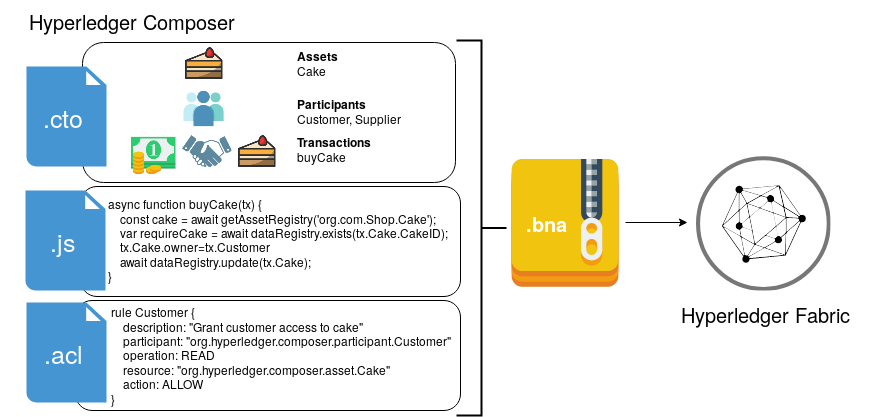
\includegraphics[width=\textwidth,height=0.45\textwidth]{img/HC.png}
        % \caption{Architecture overview}
        % \label{fig:arOv}
    \end{figure}
\end{frame}

\begin{frame}{Hyperledger Fabric network}{Chaincode}
    We use Hyperledger Composer to define our customize chaincode.
    \setbeamercovered{transparent}
    \begin{itemize}
        \onslide<1->{\item[1.]Participants, Assets
              \begin{itemize}
                  \uncover<2->{\item The data contributors represented as \textbf{DataPublisher} object.}
                        \pause
                        \pause
                        \onslide<3->{\lstinputlisting[language=modelLang]{code/Publisher.txt}}
                        \uncover<4->{\item The metadata of the data sets represented as \textbf{Data} object.}
                        \pause
                        \pause
                        \onslide<5->{\lstinputlisting[language=modelLang]{code/Data.txt}}
              \end{itemize}
              }
    \end{itemize}
\end{frame}
\begin{frame}{Hyperledger Fabric network}{Chaincode}
    \setbeamercovered{transparent}
    \begin{itemize}
        \onslide<1->{\item[2.]Transactions
              \begin{itemize}
                  \uncover<2->{\item Publish the data sets process: \textbf{AddAsset()}, \textbf{PublishData()}}
                        \pause
                        \pause
                        \onslide<3->{\lstinputlisting[language=modelLang]{code/PublishData.txt}}
                        \uncover<4->{\item Modify and Verify the data sets process: \textbf{ModifyData()} \textbf{VerifyData()}}
                        \pause
                        \pause
                        \onslide<5->{\lstinputlisting[language=modelLang]{code/ModifyData.txt}}
              \end{itemize}
              }
    \end{itemize}
\end{frame}
\begin{frame}{Hyperledger Fabric network}{Chaincode}
    \setbeamercovered{transparent}
    \begin{itemize}
        \onslide<1->{\item[3.]Access control
              \begin{itemize}
                  \uncover<2->{\item The data contributor permission.}
                        \uncover<3->{\item The citizens permission.}
                        \pause
                        \pause
                        \pause
                        \onslide<4->{\lstinputlisting[language=modelLang]{code/ACL.txt}}
              \end{itemize}
              }
    \end{itemize}
\end{frame}
\begin{frame}{Hyperledger Fabric network}{Endorsement Policy}
    \begin{itemize}
        \item[4.]Endorsement Policy
              \lstinputlisting[language=modelLang]{code/EP.txt}
    \end{itemize}
\end{frame}
\begin{frame}{Open data portal}
    \setbeamercovered{transparent}
    \onslide<1->{
        \textbf{Server-side} implementation:
        \begin{itemize}
            \uncover<2->{\item Written by NodeJS.}
                  \uncover<3->{\item Using Hyperledger Composer to interact with Hyperledger Fabric blockchain network.}
                  \uncover<4->{\item Connecting to IPFS network.}
        \end{itemize}}
    \pause
    \pause
    \pause
    \pause
    \onslide<5->{
        \textbf{Client-side} implementation:
        \begin{itemize}
            \uncover<6->{\item  Written by VueJS.}
        \end{itemize}}
\end{frame}